%%%%%%%%%%%%%%%%%%%%%%%%%%%%%%%%%%%%%%%%%%%%%%%%%%%%%%%%%%%%%%%%%%%%%%%%%%%%%%%

\chapter{RESULTADOS E DISCUSSÃO}

A Figura \ref{fig:result} é o resultado da aplicação da FFT sobre os dados de F10.7. O espectro de potência produzido é exibido normalizado pelo tamanho da série, e somente metade dos coeficientes é mostrado (visto que o output é simétrico). A Figura \ref{fig:result_t} é o mesmo resultado em função do tempo.

\begin{figure}[ht!]
	\caption{Resultado da análise espectral.}
	\vspace{1mm}	% acrescentar o espaçamento vertical apropriado entre o título e a borda superior da figura
	\begin{center}
		\resizebox{\textwidth}{!}{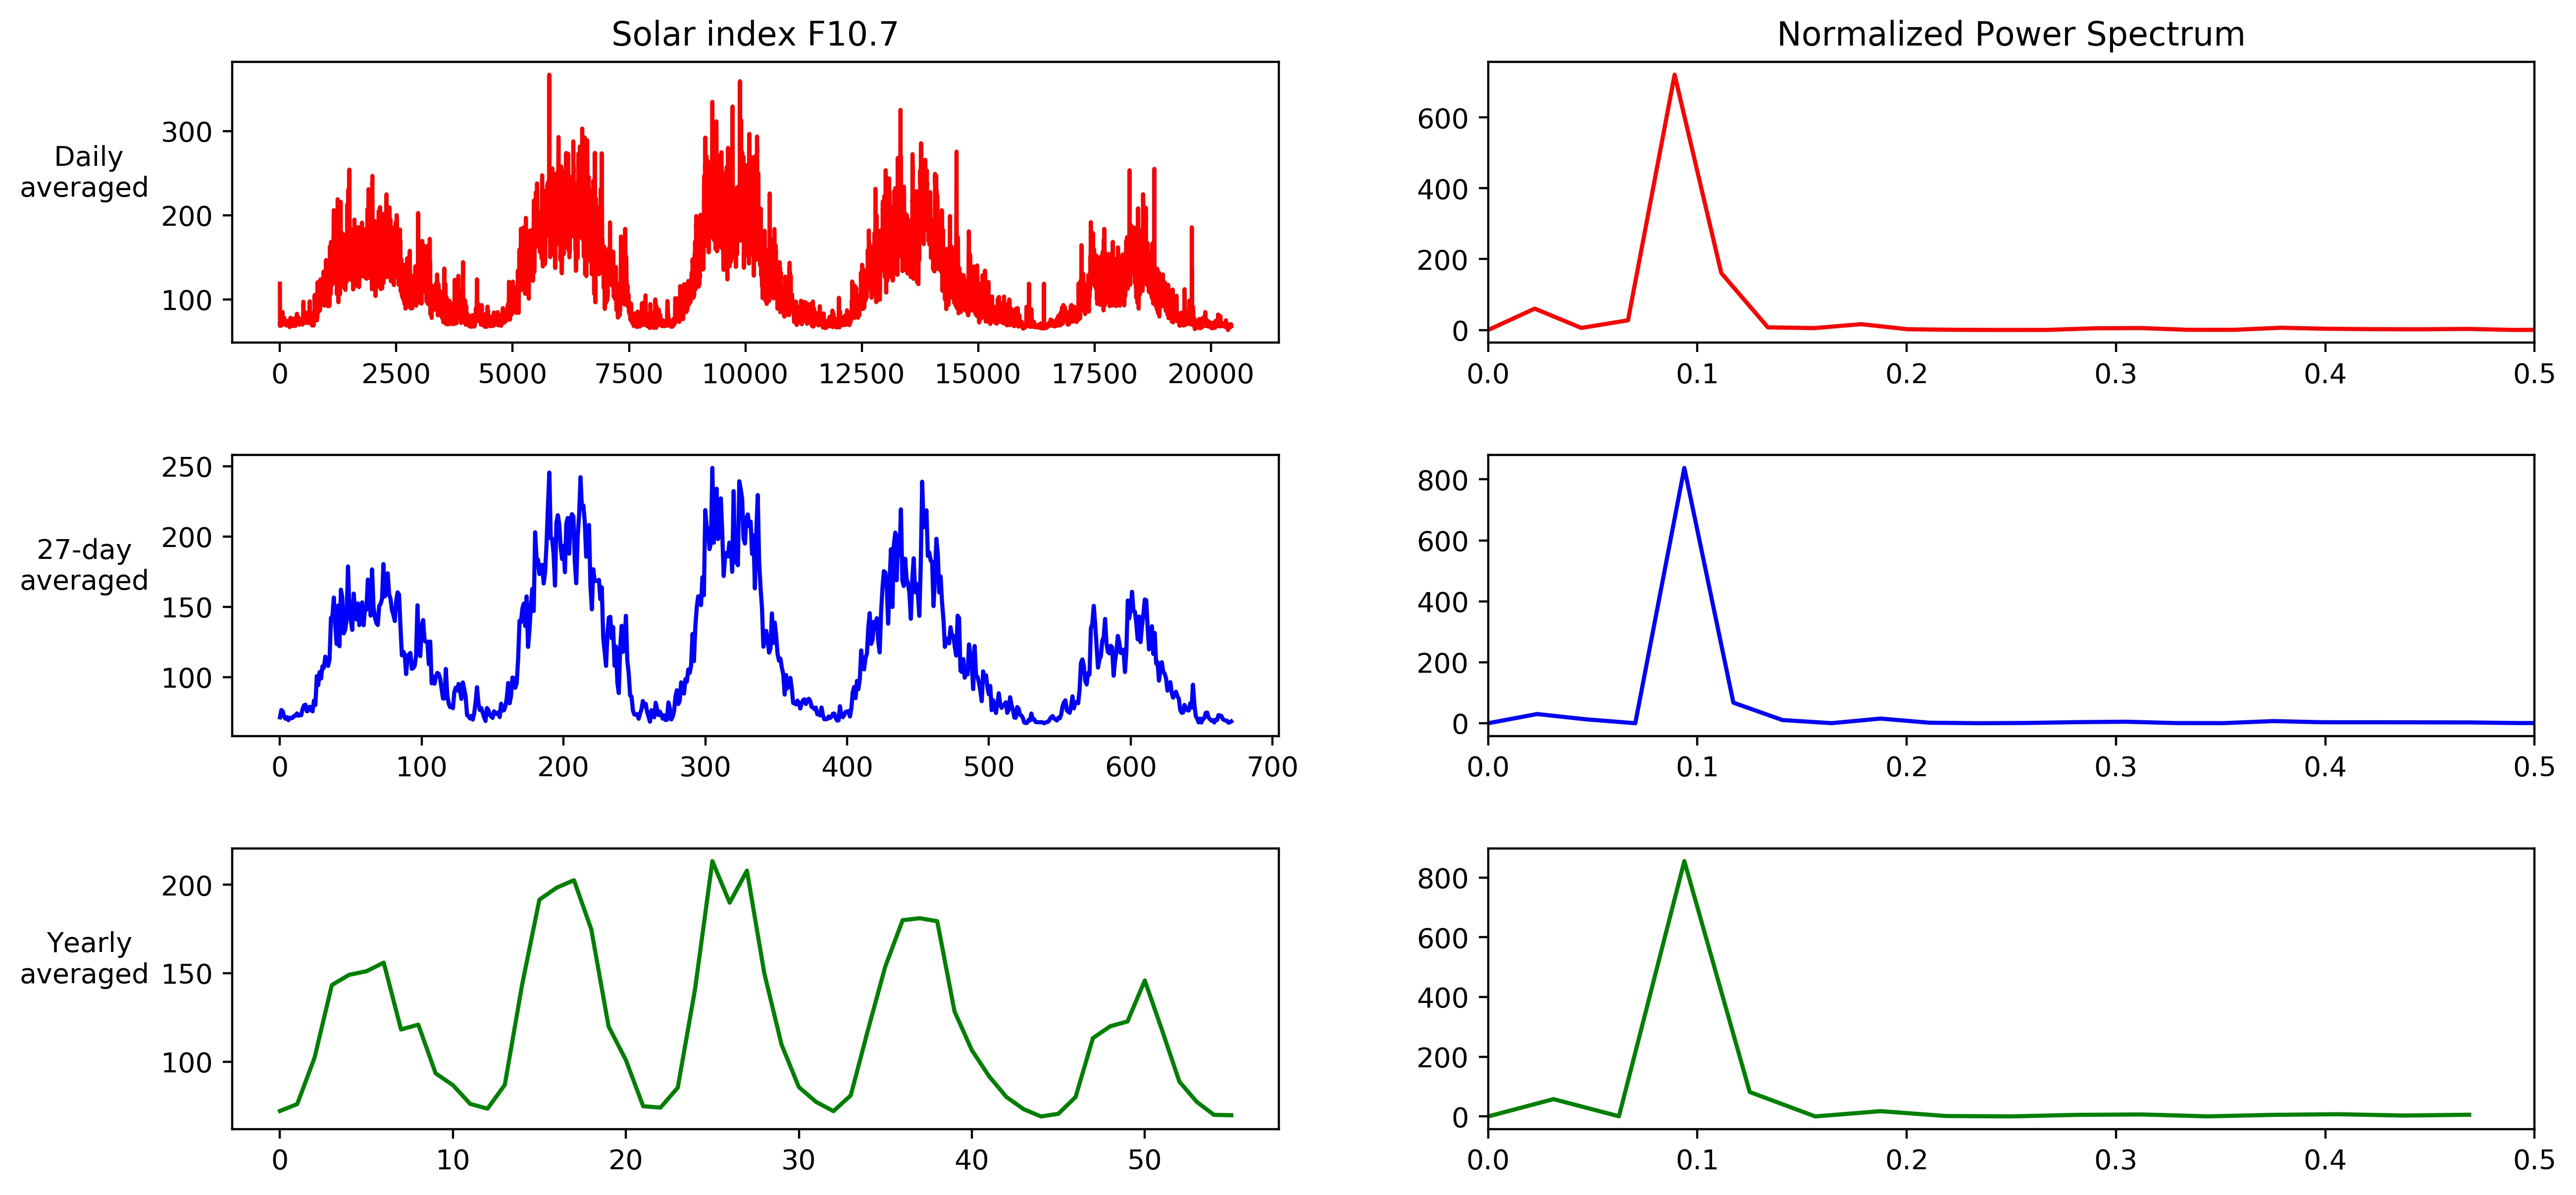
\includegraphics{Figuras/final_f.jpg}}
	\end{center}
	\vspace{1mm}	% acrescentar o espaçamento vertical apropriado entre a borda inferior da figura e a legenda ou a fonte quando não há legenda (o valor pode ser negativo para subir)
	\legenda{À esquerda, dados do fluxo solar com média diária (vermelho, cima), de 27 dias (azul, meio) e anual (verde, abaixo). À direita, resultado do espectro de potência normalizado dos respectivos sinais à esquerda. Somente metade dos coeficientes são exibidos, visto que o output é simétrico. O resultado indica que o pico da atividade solar ocorre em frequências baixas (em ciclos mais longos que um ano).}	% legenda - para deixar sem legenda usar comando \legenda{} (nunca deve-se comentar o comando \legenda)
	\label{fig:result}
	%\FONTE{\url{https://omniweb.gsfc.nasa.gov/form/dx1.html}.}	% fonte consultada (elemento obrigatório, mesmo que seja produção do próprio autor)
\end{figure}

\begin{figure}[ht!]
	\caption{Resultado em função do tempo.}
	\vspace{1mm}	% acrescentar o espaçamento vertical apropriado entre o título e a borda superior da figura
	\begin{center}
		\resizebox{\textwidth}{!}{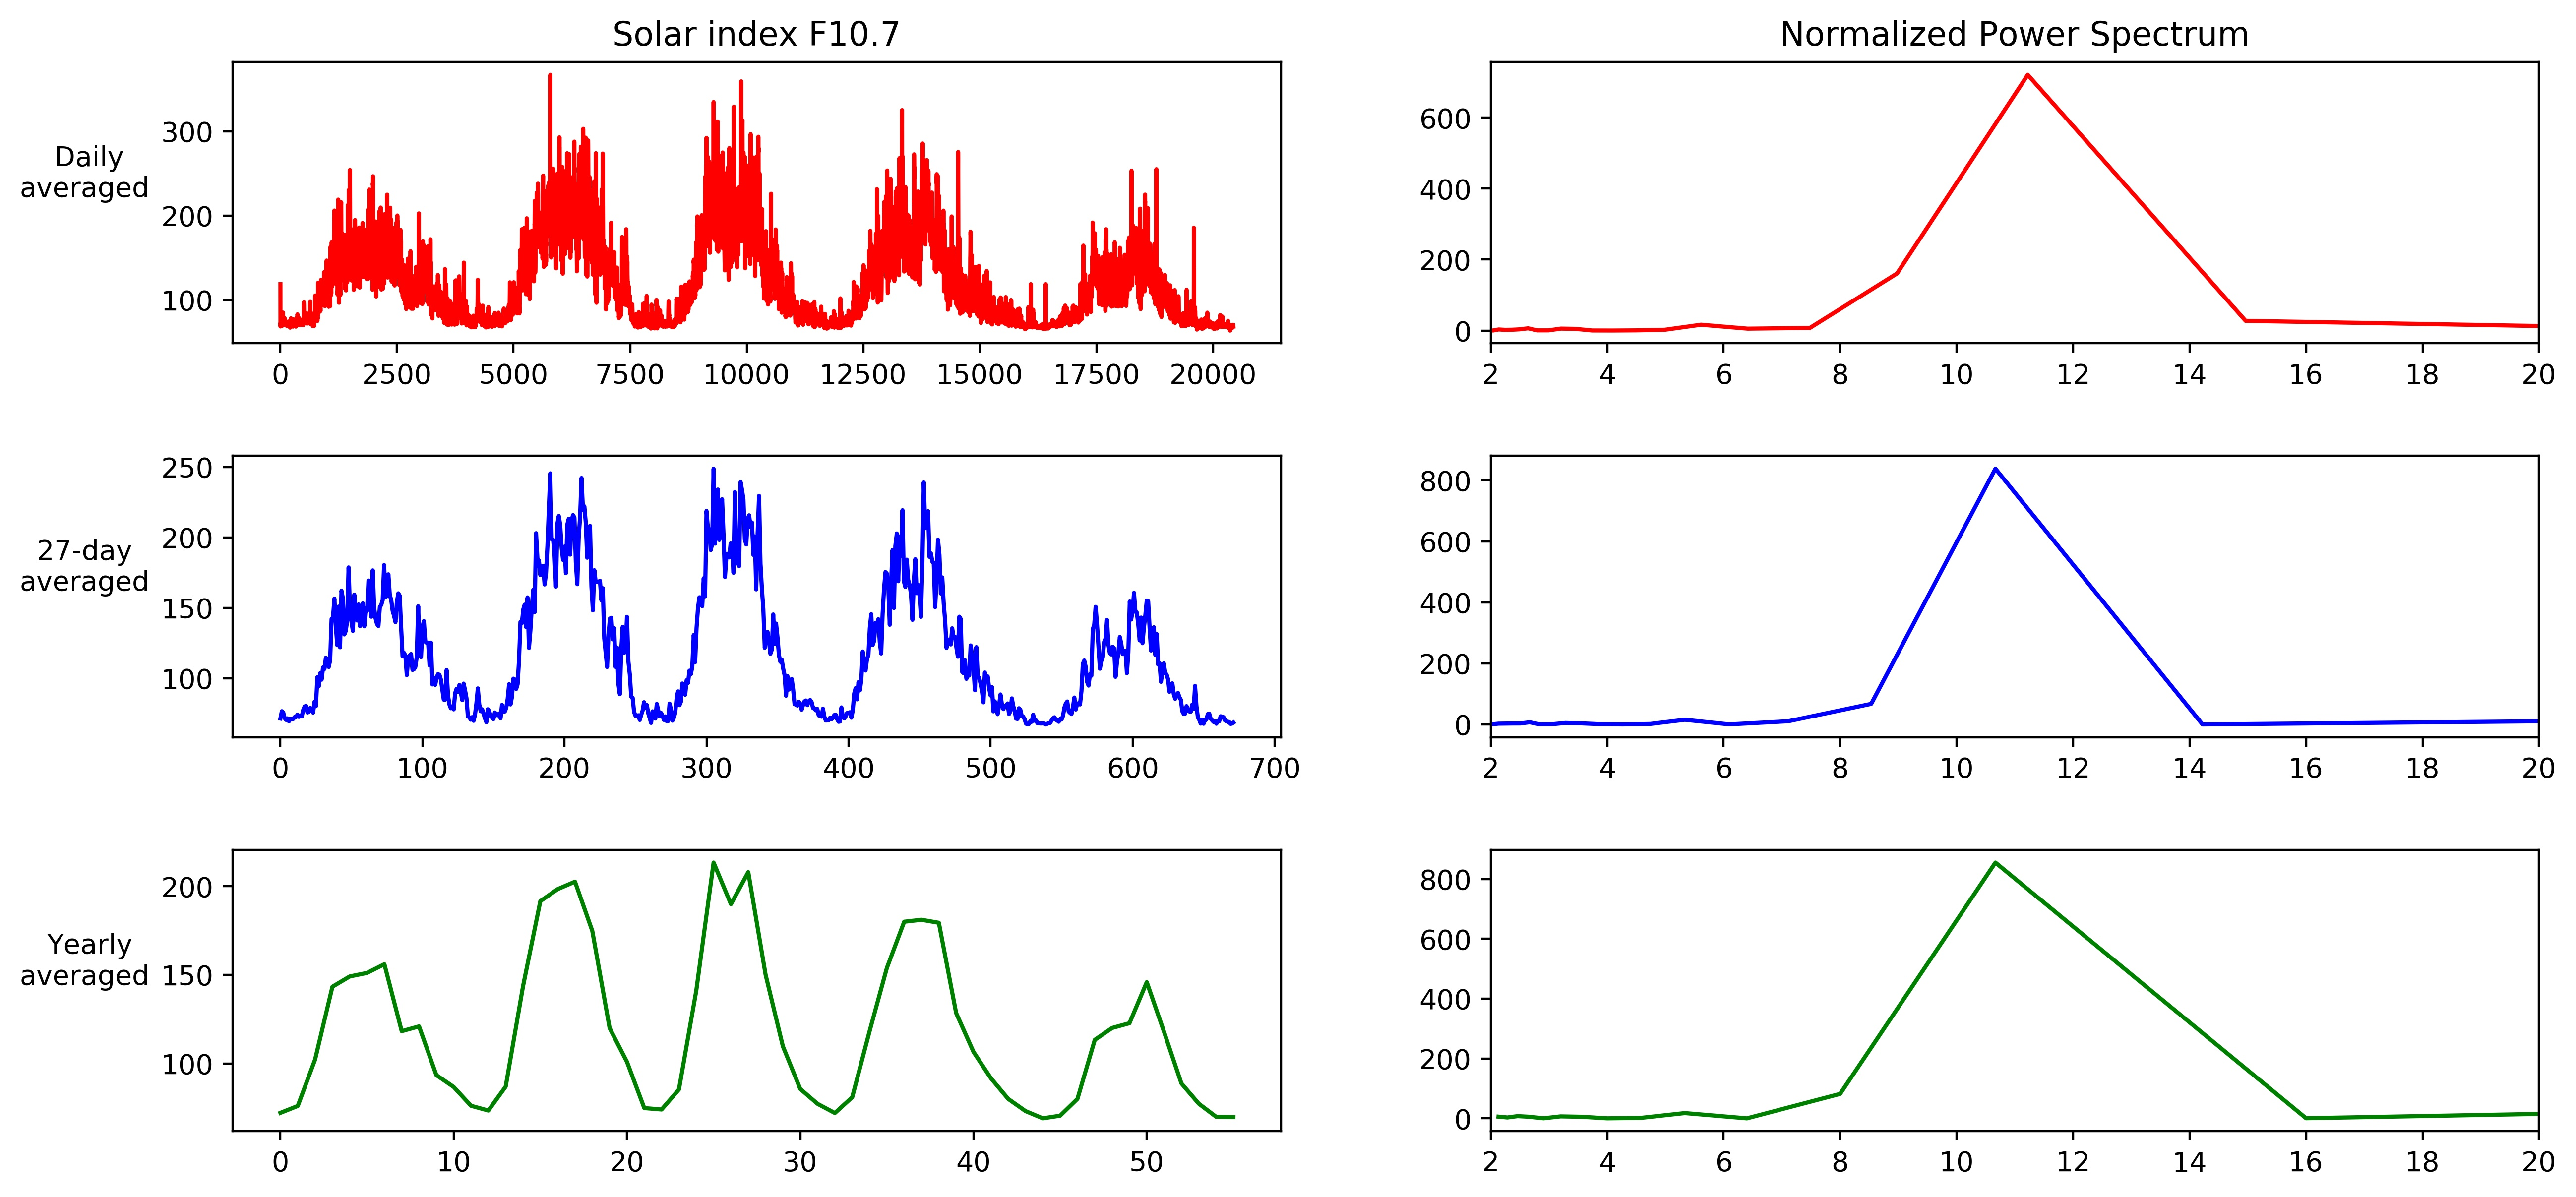
\includegraphics{Figuras/final_t2.jpg}}
	\end{center}
	\vspace{1mm}	% acrescentar o espaçamento vertical apropriado entre a borda inferior da figura e a legenda ou a fonte quando não há legenda (o valor pode ser negativo para subir)
	\legenda{Espectro de potência em função do período. O pico de atividade solar ocorre aproximadamente a cada onze anos.}	% legenda - para deixar sem legenda usar comando \legenda{} (nunca deve-se comentar o comando \legenda)
	\label{fig:result_t}
	%\FONTE{\url{https://omniweb.gsfc.nasa.gov/form/dx1.html}.}	% fonte consultada (elemento obrigatório, mesmo que seja produção do próprio autor)
\end{figure}

A principal diferença entre os três conjuntos de dados explorados está no tamanho da série. Por representarem o mesmo período temporal, pode-se interpretar que são registros do mesmo fenômeno em diferentes taxas de aquisição de dados (ou \textit{sampling}). Uma análise da Figura \ref{fig:result} indica que a média diária, o conjunto de dados de maior tamanho (2$^{14}$ entradas após tratamento) foi capaz de indicar a assinatura de frequências do sinal tão bem quanto os demais conjuntos (a média de 27 dias teve seu tamanho reduzido para 2$^{9}$ registros e a média anual para 2$^{5}$ após os procedimentos de tratamento discutidos na Seção 2). Isto deve-se ao fato de que todos os dados fazem parte de uma série histórica longa o suficiente (55 anos) para captar a assinatura do ciclo, e por isso a análise espectral é igualmente robusta para os três conjuntos analisados. E, conforme esperado, os resultados da Figura \ref{fig:result_t} indicam um ciclo de aproximadamente onze anos da atividade solar, um valor verificado na literatura e obtido também através da análise da variação do número de manchas solares. 
